\chapter{Studi Literatur}

Bab ini menjelaskan metrik evaluasi, penelitian terkait, dan perkembangan representasi teks lintas bahasa mulai dari teknik-teknik terdahulu hingga yang terbaru menggunakan \textit{language model pretraining} lintas bahasa. 

\section{Representasi Teks Lintas Bahasa}
    Salah satu bentuk dari Transfer Learning adalah pembelajaran lintas bahasa \parencite{ruder2019transfer}. Pada pembelajaran lintas bahasa, pembelajaran pertama-tama dilakukan di bahasa lain yang lebih populer dan kemudian digunakan pada bahasa lain yang lebih tidak populer. Untuk dapat melakukan hal ini, diperlukan representasi bahasa pada ruang yang sama seperti dapat dilihat pada ilustrasi di gambar \ref{fig:ilustrasi_embedding}.

    \begin{figure}[ht]
        \centering
        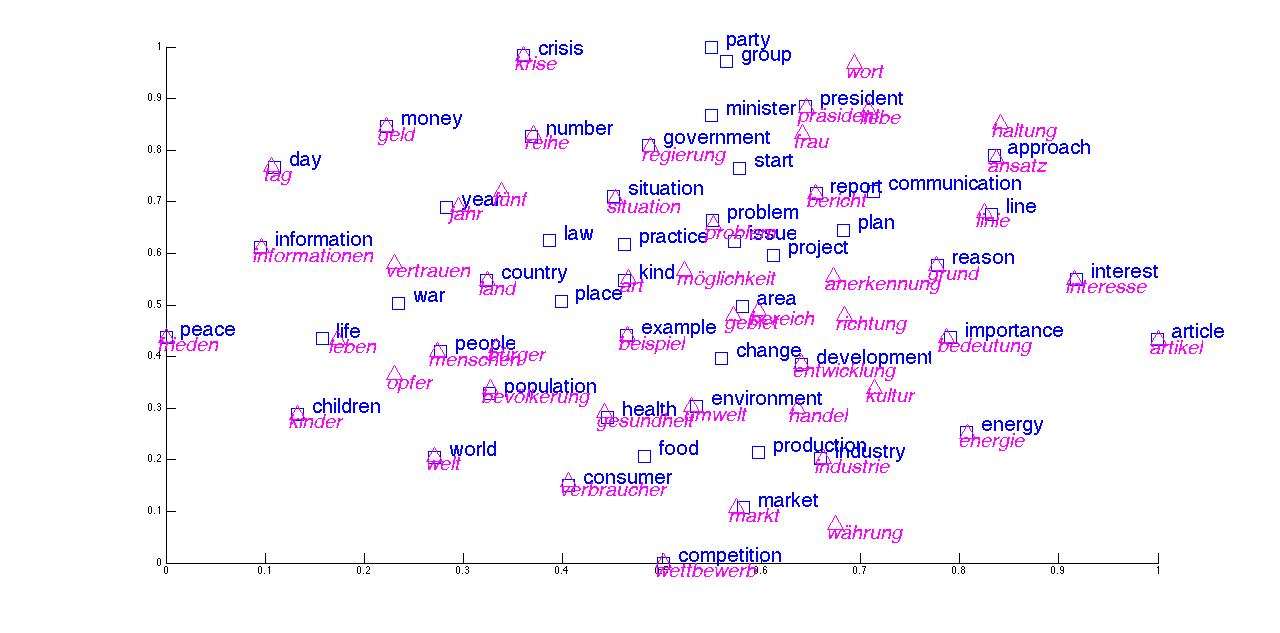
\includegraphics[width=1\textwidth]{resources/luong_et_al_2015.jpg}
        \caption{Ilustrasi ruang \textit{embedding} antara dua bahasa \parencite{Luong_Pham_Manning_2015}}
        \label{fig:ilustrasi_embedding}
    \end{figure}

    Sebelumnya, diperlukan ahli untuk membangun kamus kata-kata dan kalimat secara manual untuk dapat membandingkan kata dari dua bahsa. Seiring dengan perkembangan teknologi, berbagai teknik berkembang untuk dapat melakukan hal ini secara otomatis. Berdasarkan \parencite{Wang_Xie_Xu_Yang_Neubig_Carbonell_2019}, secara garis besar terdapat 2 pendekatan berbeda dalam membangun ruang \textit{embedding} antar bahasa:

    \begin{enumerate}
        \item \textit{Monolingual mapping}: Pada teknik ini, model dilatih secara independen pada bahasa masing-masing. Kemudian mapping antara bahasa dipelajari untuk mendapatkan representasi antar bahasa.

        \item \textit{Joint optimization}: Pada teknik ini, model dilatih pada korpus antar bahasa. Model kemudian mengoptimisasi kombinasi dari monolingual dan cross-lingual loss.
    \end{enumerate}

    Pada \textit{monolingual mapping}, salah satu teknik adalah dengan pertama-tama mempelajari representasi bahasa menggunakan model Skip-gram atau Continuous Bag-of-Words (CBOW) yang didistribusikan diusulkan oleh \parencite{MikolovEstimation}. Model-model ini mempelajari representasi kata menggunakan arsitektur \textit{neural network} sederhana yang bertujuan untuk memprediksi tetangga kata. Karena kesederhanaannya, model Skip-gram dan CBOW dapat dilatih pada sejumlah besar data teks. Pada implementasi paralelnya model ini dapat belajar dari miliaran kata dalam hitungan jam.

    Baru-baru ini ditunjukkan bahwa representasi kata yang didistribusikan secara mengejutkan menangkap banyak keteraturan linguistik, dan ada banyak jenis kesamaan di antara kata-kata yang dapat dinyatakan sebagai terjemahan linear \parencite{MikolovLinguistic2013}. Misalnya, operasi vektor "raja" - "pria" + "wanita" menghasilkan vektor yang dekat dengan "ratu".

    Dua model khusus untuk mempelajari representasi kata yang dapat dilatih secara efisien pada banyak data teks adalah model Skip-gram dan CBOW yang diperkenalkan di \parencite{MikolovEstimation}. Dalam model CBOW, tujuan pelatihannya adalah untuk menggabungkan representasi kata di sekitarnya untuk memprediksi kata di tengah. Sedangkan dalam model Skip-gram, tujuan pelatihan adalah untuk mempelajari representasi kata vektor yang pandai memprediksi konteksnya dalam kalimat yang sama \parencite{MikolovEstimation}. Model arsitektur dari dua metode ini ditunjukkan pada Gambar \ref{fig:ilustrasi_cbow_skip_gram}.

    \begin{figure}[ht]
        \centering
        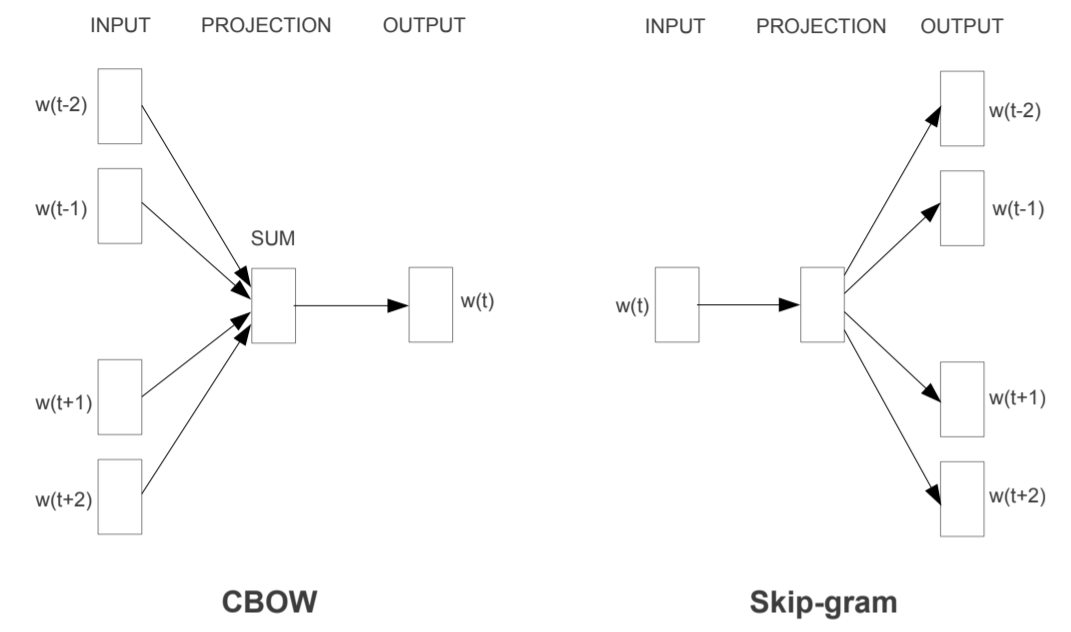
\includegraphics[width=1\textwidth]{resources/cbow-skip-gram-illustration.png}
        \caption{Ilustrasi model CBOW dan Skip-gram. \parencite{MikolovExploiting}.}
        \label{fig:ilustrasi_cbow_skip_gram}
    \end{figure}
    
    Lebih formal, diberi urutan kata pelatihan \(w1, w2, w3,. . . , wT,\) tujuan dari model Skip-gram adalah untuk memaksimalkan probabilitas log rata-rata

    \begin{equation}
        \frac{1}{T}\sum_{t=1}^{T}\begin{bmatrix}
        \sum_{j=-k}^{K}{\log p(w_{t+j}|w_{t})}
        \end{bmatrix}
        \label{eq:1}
    \end{equation}

    di mana \(k\) adalah ukuran jendela pelatihan. Iterasi penjumlahan di bagian dalam berjalan dari \({-k}\) ke \(k\) untuk menghitung probabilitas log benarnya memprediksi kata \(w_{t+j}\) jika kata di tengah \(w_{t}\). Iterasi penjumlahan di luar mencakup semua kata dalam korpus pelatihan. 

    % TODO: Lanjutin penjelasan Skip-gram dari Mikolov: Expoiting
    %Dalam model Skip-gram, setiap kata w dikaitkan dengan dua vektor parameter yang dapat dipelajari, \(u_{w}\) dan \(v_{w}\). Vektor ini adalah vektor "\textit{input}" dan "\textit{output}" dari \(w\) masing-masing. Peluang untuk memprediksi kata dengan benar dengan kata "wj" didefinisikan sebagai

    Ketika dilatih tentang dataset besar, model Skip-gram atau CBOW ini menangkap banyak informasi semantik. Seperti yang disebutkan sebelumnya, kata-kata yang berkaitan erat memiliki representasi vektor yang serupa, misalnya, sekolah dan universitas, danau, dan sungai. Ini karena sekolah dan universitas muncul dalam konteks yang sama, sehingga selama pelatihan representasi vektor dari kata-kata ini didorong untuk menjadi dekat satu sama lain. Lebih menarik lagi, vektor menangkap hubungan antara konsep melalui operasi linier. Misalnya, \(vektor(Prancis) - vektor(Paris)\) mirip dengan \(vektor(Italia) - vektor(Roma)\).

    Pada gambar \ref{fig:ilustrasi_embedding_inggris_spanyol}, dapat dilihat visualisasi hasil pembelajaran Skip-gram atau CBOW. Gambar \ref{fig:ilustrasi_embedding_inggris_spanyol} memvisualisasikan vektor untuk angka dan hewan dalam bahasa Inggris dan Spanyol, dan dapat dengan mudah dilihat bahwa konsep-konsep ini memiliki susunan geometris yang serupa. Hal ini dikarenakan semua bahasa umum memiliki konsep yang didasarkan pada dunia nyata (seperti kucing adalah binatang yang lebih kecil dari seekor anjing), sering kali ada kesamaan kuat antara ruang vektor. Kesamaan pengaturan geometris dalam ruang vektor adalah alasan utama mengapa metode ini dapat bekerja dengan baik.

    \begin{figure}[ht]
        \centering
        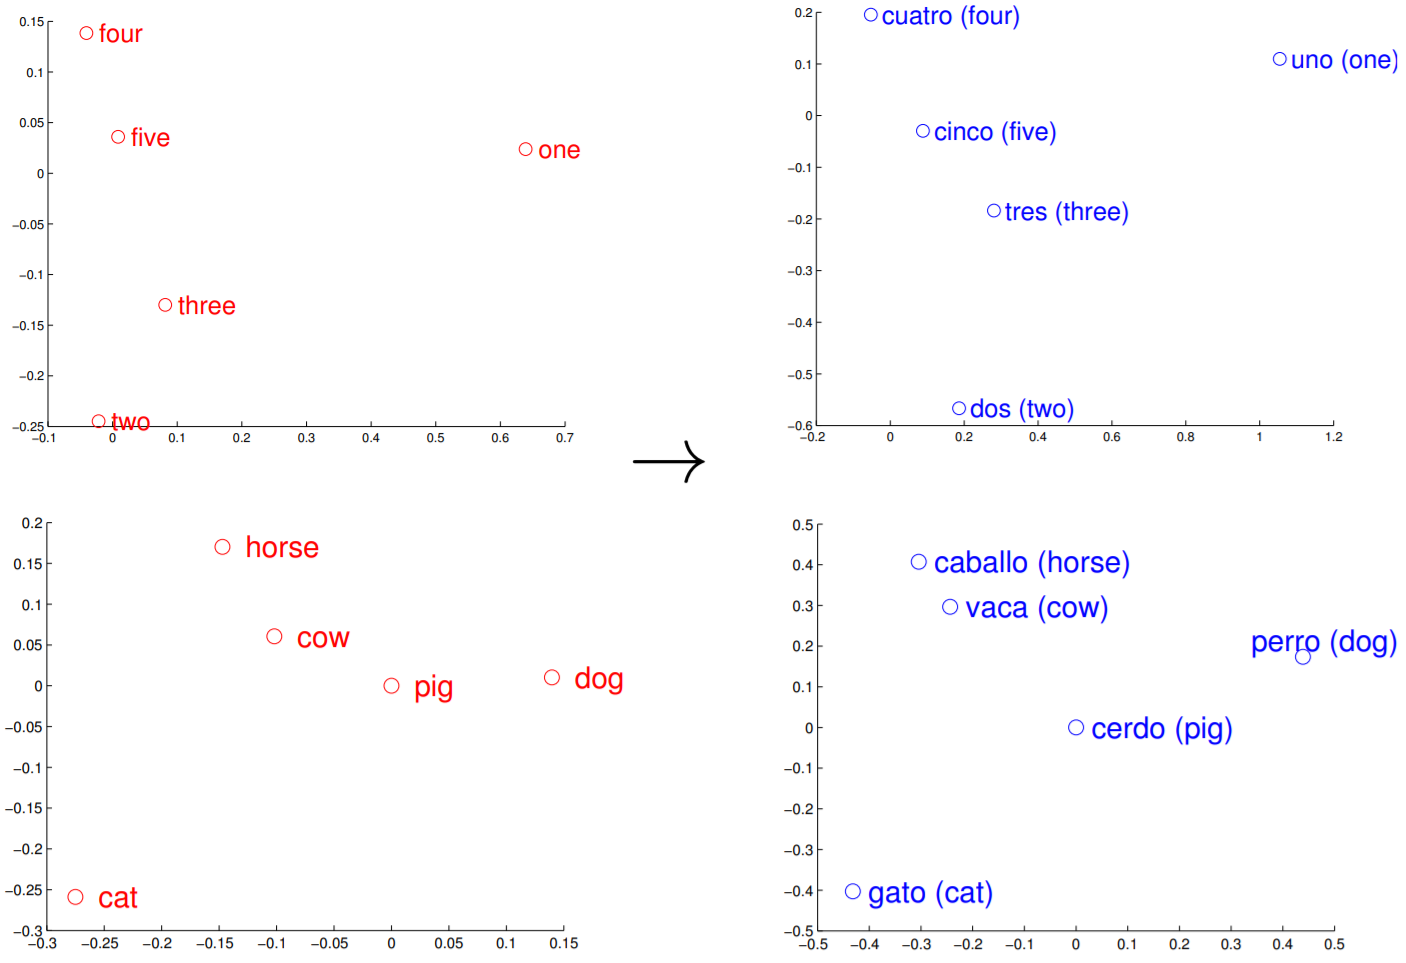
\includegraphics[width=1\textwidth]{resources/ilustration-eng-spn-word.png}
        \caption{Ilustrasi ruang \textit{embedding} antara bahasa Inggris dan Spanyol \parencite{MikolovExploiting}.}
        \label{fig:ilustrasi_embedding_inggris_spanyol}
    \end{figure}

    Dikarenakan miripnya representasi bahasa, jika translasi beberapa objek diketahui, contoh angka satu sampai lima, representasi antar bahasa dapat disesuaikan dengan rotasi, \textit{scaling}, dan translasi untuk mendapatkan tranlasi angka lainnya. Lebih formalnya, misalkan diberi satu set pasangan kata dan representasi vektor yang terkait \begin{math} \begin{Bmatrix} {x_{i}, z_{i}} \end{Bmatrix}_{i=1}^{n} \end{math}, di mana \(x_{i}\in\mathbb{R}^{d_{1}}\) adalah representasi terdistribusi dari kata i dalam bahasa sumber, dan \(z_{i}\in\mathbb{R}^{d_{2}}\) adalah representasi vektor dari terjemahannya. Kemudian dicari matriks transformasi \( W\) sehingga \(W x_{i}\) mendekati \(z_{i}\). Dalam praktiknya, \(W\) dapat dipelajari dengan masalah optimasi berikut

    \begin{equation}
        \min_{W}\sum_{i=1}^{n}\left \| Wx_i-z_i \right \|^2
        \label{eq:2}
    \end{equation}

    yang dapat diselesaikan dengan \textit{stochastic gradient descent} \parencite{MikolovExploiting}.

    Setiap kata baru yang diberikan dan representasi vektor kontinu \(x\) dapat dipetakan ke ruang bahasa lain dengan menghitung \(z = W x\) pada saat prediksi. Kemudian kata yang representasinya paling dekat dengan \(z\) dalam ruang bahasa target dapat ditemukan menggunakan \textit{cosine similarity} sebagai metrik jarak. Terlepas dari kesederhanaannya, metode transformasi linier ini bekerja dengan baik dalam eksperimen yang \parencite{MikolovExploiting} jalankan, lebih baik daripada teknik \textit{nearest neighbour} dan juga pengklasifikasi \textit{neural network}.

    Meski \textit{monolingual mapping} sukses mendapatkan ruang \textit{embedding} antar bahasa, teknik ini mahal dan susah diaplikasikan ke bahasa yang memiliki sumber daya rendah. Untuk dapat mengaplikasikan teknik ini diperlukan kamus kata-kata atau kalimat paralel antar bahasa, hal yang seringkali tidak tersedia pada bahasa bersumber daya rendah. Oleh karena itu, mengaplikasikan teknik ini sangat sulit pada bahasa Indonesia. 

    Kemajuan terbaru datang dari teknik \textit{joint optimization}. Teknik \textit{joint optimization} yang sebelumnya memerlukan korpus paralel atau kamus bilingual (\textit{supervised}) \parencite{Xing_Wang_Liu_Lin}, kini dapat dilakukan tanpa korpus paralel atau kamus bilingual (\textit{unsupervised}) \parencite{LampleConneau2019}. Hal ini dilakukan dengan memanfaatkan \textit{shared sub-word vocabulary}. Tidak hanya itu, \parencite{LampleConneau2019} juga memanfaatkan \textit{masked language modeling} dan arsitektur \textit{transformer} untuk mendapatkan \textit{language model} yang mangkus. Sub-bab selanjutnya akan membahas detail \textit{shared sub-word vocabulary}, \textit{masked language modeling}, dan arsitektur \textit{transformer} dari \textit{language model pretraining} lintas bahasa bernama XLM yang dikembangkan oleh \parencite{LampleConneau2019}.

% \section{ \textit{Language Model Pretraining} Lintas Bahasa}
\section{Language Model Pretraining Lintas Bahasa}
    Seperti yang dijelaskan sebelumnya, penelitian \parencite{LampleConneau2019} mendemonstrasikan pembangunan \textit{language model pretraining} lintas bahasa yang dilakukan tanpa memerlukan korpus paralel atau kamus bilingual. Bab ini akan menjelaskan bagian-bagian dari \textit{language model} yang diberi nama XLM ini yaitu \textit{shared sub-word vocabulary}, \textit{masked language modeling}, arsitektur \textit{transformer}, dan teknik \textit{pretraining}.

    \subsection{Arsitektur Transformer}

    Berdasarkan \parencite{AttentionVaswani2017}, arsitektur \textit{Transformer} terdiri dari \textit{self-attention} dan \textit{point-wise} yang ditumpuk, dan \textit{fully connected layer} untuk enkoder dan dekoder. Ilustrasi secara keseluruhan arsitektur \textit{Transformer} dapat dilihat pada Gambar \ref{fig:ilustrasi_transformer}.

    \begin{figure}[ht]
        \centering
        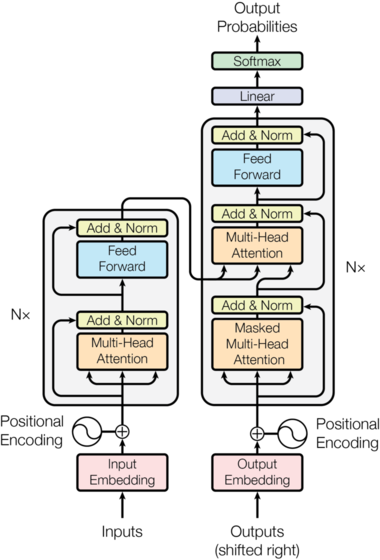
\includegraphics[width=0.4\textwidth]{resources/overview-transformer.png}
        \caption{Ilustrasi \textit{transformer} secara keseluruhan \parencite{AttentionVaswani2017}.}
        \label{fig:ilustrasi_transformer}
    \end{figure}

    Fungsi \textit{attention} dapat digambarkan sebagai memetakan kueri dan pasangan \textit{key-value} untuk suatu output, di mana kueri (Q), kunci (K), nilai (V), dan \textit{output} semuanya vektor. \textit{Output} dihitung sebagai \textit{weighted sum} dari nilai-nilai, di mana bobot yang ditetapkan untuk setiap nilai dihitung oleh fungsi kompatibilitas kueri dari kunci yang sesuai.

    Pada penelitian \parencite{AttentionVaswani2017}, tipe \textit{attention} ini disebut "\textit{Scaled Dot-Product Attention}". Input terdiri dari kueri dan kunci dimensi \(d_{k}\), dan nilai dimensi \(d_{v}\). \textit{Dot product} dari kueri dihitung dengan semua kunci, membaginya dengan \(\sqrt{d_{k}}\), dan menerapkan fungsi softmax untuk mendapatkan bobot pada nilai. Ilustrasi \textit{attention} dapat dilihat pada Gambar \ref{fig:ilustrasi_attention}.

    \begin{figure}[ht]
        \centering
        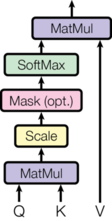
\includegraphics[width=0.2\textwidth]{resources/overview-attention.png}
        \caption{Ilustrasi \textit{attention} secara keseluruhan \parencite{AttentionVaswani2017}.}
        \label{fig:ilustrasi_attention}
    \end{figure}

    Pada prakteknya, hasil keluaran fungsi \textit{attention} pada sebuah set kueri dihitung secara besamaan, dikemas bersama menjadi matriks Q. Kunci dan nilai juga dikemas bersama menjadi matriks K dna V. Kemudian hasil keluaran dapat dihitung dengan:

    \begin{equation}
        Attention(Q,K,V) = softmax(\frac{QK^{T}}{\sqrt{d_k}})V
    \end{equation}

    Pada model XLM yang akan digunakan di tugas akhir ini, digunakan model dengan 12-\textit{layer Transformer}. Arsitektur model ini sama dengan arsitektur model yang digunakan \parencite{LampleConneau2019} untuk melakukan klasifikasi pada data tolak ukur XNLI.

    \subsection{Shared sub-word vocabulary}
    % \subsection{\textit{Shared sub-word vocabulary}}
    Berdasarkan penelitian oleh \parencite{Sennrich_Haddow_Birch_2016}, salah satu inspirasi menggunakan \textit{sub-word} adalah fakta bahwa terjemahan beberapa kata bersifat transparan karena terjemahannya dapat diterjemahkan oleh penerjemah yang kompeten, bahkan jika itu adalah kata yang belum pernah ditemui, berdasarkan terjemahan dari \textit{sub-word} yang dikenal seperti morfemnya atau fonemnya. Kategori kata yang terjemahannya berpotensi transparan meliputi:

    \begin{enumerate}
        \item Entitas bernama (\textit{named entities}). Di antara bahasa yang menggunakan alfabet, nama seringkali dapat disalin dari sumber ke teks target. Transkripsi atau transliterasi mungkin diperlukan pada bahasa dengan huruf atau suku kata berbeda. Contoh: \\
        Barack Obama (Bahasa Inggris dan Jerman) \\
        \foreignlanguage{russian}{Барак Обама} (Bahasa Rusia) \\
        \begin{CJK}{UTF8}{min}
        バラク・オバマ (ba-ra-ku o-ba-ma) (Bahasa Jepang)
        \end{CJK}

        \item Kata-kata serumpun dan pinjaman. Kata serumpun dan kata pinjaman dengan asal yang sama dapat berbeda secara reguler antar bahasa, sehingga aturan penerjemahan tingkat karakter sudah cukup \parencite{Tiedemann2012}. Contoh:  \\
        claustrophobia (Bahasa Inggris) \\
        Klaustrophobie (Bahasa Jerman) \\
        \foreignlanguage{russian}{Клаустрофобия} (Klaustrofobiâ) (Bahasa Rusia)

        \item Kata-kata yang rumit secara morfologis. Kata-kata yang mengandung banyak morfem, misalnya yang dibentuk melalui peracikan, afiksasi, atau infleksi, dapat diterjemahkan dengan menerjemahkan morfem secara terpisah. Contoh:  \\
        solar system (Bahasa Inggris) \\
        Sonnensystem (Sonne + System) (Bahasa Jerman) \\
        Naprendszer (Nap + Rendszer) (Bahasa Hongaria)
    \end{enumerate}

    Penelitian \parencite{Sennrich_Haddow_Birch_2016} membuktikan bahwa segmentasi kata-kata langka ke dalam unit \textit{sub-word} yang sesuai sudah cukup untuk memungkinkan \textit{neural translation network} mempelajari terjemahan yang transparan, dan menggeneralisasikan pengetahuan ini untuk menerjemahkan dan menghasilkan kata-kata yang tidak ditemui sebelumnya. Pada penelitiannya, mereka menggunakan teknik \textit{Byte Pair Encoding} untuk mendapatkan tidak hanya \textit{sub-word}-nya tetapi juga kompresi dari kamus-kamus kata yang ada.

    Teknik \textit{Byte Pair Encoding} (BPE) \parencite{GageBPE1994} adalah teknik kompresi data sederhana yang secara iteratif menggantikan pasangan \textit{byte} yang paling sering muncu; secara berurutan dengan \textit{byte} tunggal yang tidak digunakan. Pada penelitiannya, \parencite{Sennrich_Haddow_Birch_2016} mengadaptasi algoritma \textit{Byte Pair Encoding} untuk segmentasi kata. Alih-alih sering menggabungkan pasangan \textit{byte}, mereka menggabungkan karakter atau urutan karakter.

    Pertama-tama, kosakata simbol diinisialisasi dengan kosakata karakter, dan mewakili setiap kata sebagai urutan karakter, ditambah simbol akhir kata khusus ‘·’, yang memungkinkan hasil terjemahan dikembalikan ke bentuk awal setelah terjemahan. Kemudian semua pasangan simbol dihitung secara iteratif dan untuk setiap pasangan yang paling sering diganti dengan simbol baru. Contoh ('A', 'B') menjadi 'AB'. Setiap operasi penggabungan menghasilkan simbol baru yang mewakili \textit{n-gram} dari karakter. Karakter yang sering muncul (atau seluruh kata) pada akhirnya digabungkan menjadi satu simbol. Ukuran kosa kata simbol akhir sama dengan ukuran kosa kata awal, ditambah jumlah operasi penggabungan --- yang merupakan satu-satunya \textit{hyperparameter} dari algoritma.

    Dapat dilihat contoh sederhana algoritma \textit{Byte Pair Encoding} pada Lampiran \ref{appendix:simple_bpe_algorithm} oleh \parencite{Sennrich_Haddow_Birch_2016}. Pada algoritma ini, operasi \textit{Byte Pair Encoding} belajar dari kamus kata {‘low’, ‘lower’, ‘newest’, ‘widest’}. Pada akhir iterasi, akan diperoleh representasi dari kamus kata dalam bentuk simbol-simbol yang dipelajari. Pada contoh tersebut, kata 'lowest' yang berada diluar kamus kata akan direpresentasikan menjadi gabungan dari simbol 'low' dan 'est'. Di sini dapat dilihat bagaimana \textit{Byte Pair Encoding} dapat membantu merepresentasikan kata yang berada diluar kamus kata. 

    \subsection{Masked Language Modeling (MLM)}
    Dideskripsikan pada penelitian oleh \parencite{Devlin_Chang_Lee_Toutanova_2019}, \textit{Masked Language Modeling} terinspirasi dari \textit{Cloze task} \parencite{Taylor_1953}. Teknik MLM secara acak akan menyembunyikan beberapa kata dari input, dan model memiliki objektif untuk menebak kata asli dari kata yang disembunyikan tadi berdasarkan konteks yang ada di sekelilingnya. Tidak seperti pelatihan \textit{language model} lainnya yang berjalan dari kiri-ke-kanan, pelatihan dengan objektif MLM memungkinkan representasi dari kiri dan kanan mengambil peran. Hal ini memungkinkan pelatihan \textit{Transformer} secara dua arah. Ilustrasi dari \textit{masked language modeling} secara keseluruhan dapat dilihat pada Gambar \ref{fig:ilustrasi_transformer}.

    \begin{figure}[ht]
        \centering
        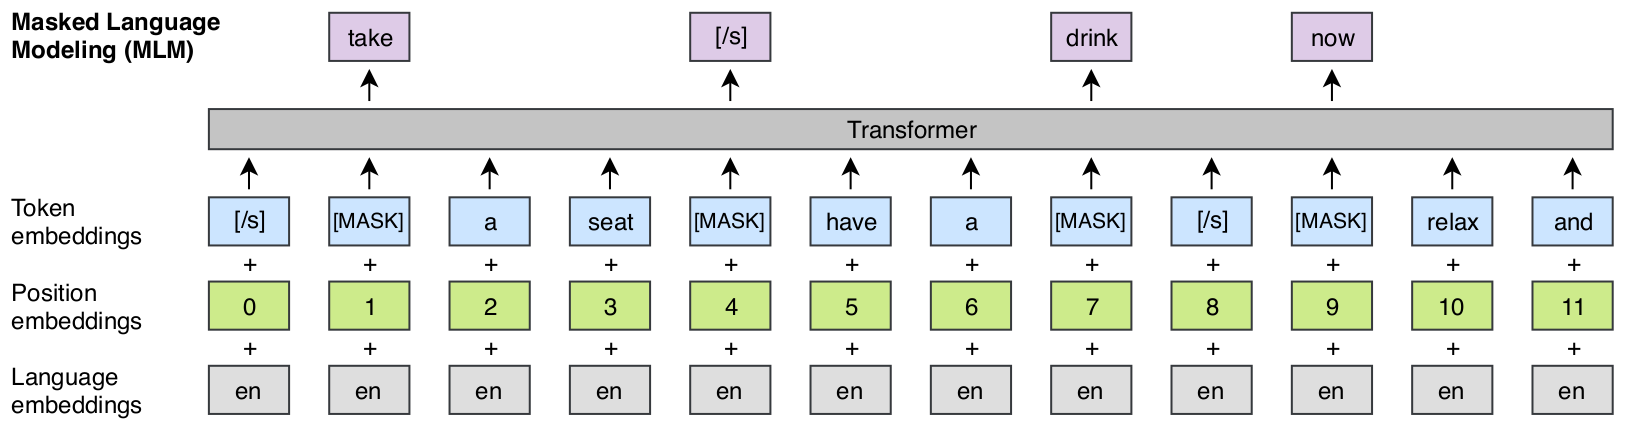
\includegraphics[width=1\textwidth]{resources/ilustrasi-mlm.png}
        \caption{Ilustrasi \textit{masked language modeling} \parencite{LampleConneau2019}.}
        \label{fig:ilustrasi_mlm}
    \end{figure}

    Sama dengan BERT, persentase dari kata yang akan dipilih untuk disembunyikan pada XLM adalah 15 persen. Setelah sebuah posisi dipilih secara acak, sebuah kata kemudian memiliki 80 persen kemungkinan untuk disembunyikan, 10 persen kemungkinan untuk diganti menjadi sebuah kata acak, dan 10 persen kemungkinan tidak diganti sama sekali.

    \subsection{Teknik Pretraining}
    Model XLM ini merupakan perkembangan dari penelitian oleh \parencite{radford2018improving}; \parencite{HowardRuder2018}; dan \parencite{Devlin_Chang_Lee_Toutanova_2019}; yang meneliti \textit{language modeling} untuk melakukan \textit{pretraining Transformer encoder}. Penelitian-penelitian tersebut sukses membuktikan mangkusnya teknik ini dengan meraih kenaikan performa yang tinggi pada dataset tolak ukur GLUE \parencite{GLUE2019}.

    Teknik \textit{language model pretraining} sukses dikarenakan kemampuannya untuk memanfaatkan data-data teks yang ada dari berbagai sumber tanpa perlu melakukan pelabelan \textit{(unsupervised)}. Pada salah satu model XLM, \textit{pretraining} dilakukan pada data Wikipedia dari 100 bahasa. Melalui pembelajaran dari Wikipedia 100 bahasa ini XLM berhasil mempelajari representasi teks berbagai bahasa.

\section{Metrik Evaluasi}
Permasalahan klasifikasi konten negatif di internet merupakan permasalahan yang memiliki kelas tidak seimbang. Dalam permasalahan seperti ini, metrik accuracy dapat menyesatkan dan mengakibatkan paradoks akurasi \parencite{Zhu_Davidson_2007}. Untuk mengevaluasi performa dari analisis sentimen yang dilakukan pada bahasa Indonesia, digunakan \textit{f1-score}. \textit{f1-score} adalah rata-rata harmonis antara precision dan recall. Berikut definisi dari \textit{precision} (II.1),  \textit{recall} (II.2),  \textit{f1-score} (II.3)  secara matematis:
\begin{equation}
    precision=\frac{True Positive}{True Positive + False Positive}
\end{equation}
\begin{equation}
    recall=\frac{True Positive}{True Positive + False Negative}
\end{equation}
\begin{equation}
    f1-score=2.\: \frac{precision\: .\: recall}{precision+recall}
\end{equation}

Dengan pengelompokan prediksi sesuai dengan \textit{confusion matrix} pada tabel \ref{tab:confusion_matrix}.
\begin{table}[ht]
    \centering
    \begin{tabular}{@{}cc|cc@{}}
    \multicolumn{1}{c}{} &\multicolumn{1}{c}{} &\multicolumn{2}{c}{Prediksi} \\ 
    \multicolumn{1}{c}{} & 
    \multicolumn{1}{c|}{} & 
    \multicolumn{1}{c}{\textit{True}} & 
    \multicolumn{1}{c}{\textit{False}} \\ 
    \cline{2-4}
    \multirow[c]{2}{*}{\rotatebox[origin=tr]{90}{Label}}
    & \textit{True}  & \textit{True Positive} & \textit{False Negative}   \\[1.5ex]
    & \textit{False}  & \textit{False Positive}   & \textit{True Negative} \\ 
    \cline{2-4}
    \end{tabular}
    \caption{Tabel \textit{Confusion matrix}.}
    \label{tab:confusion_matrix}
\end{table}

\section{Penelitian Terkait}
Sebelumnya telah banyak penelitian terkait baik analisis sentimen maupun pembelajan lintas bahasa. \textbf{Pada penelitian \parencite{FarhanKhodra2017}} yang berjudul “\textit{Sentiment-specific word embedding for Indonesian sentiment analysis}”, berbagai bentuk representasi teks dibandingkan dan dievaluasi menggunakan dataset ulasan TripAdvisor. Hasil dari penelitian ini dapat dilihat pada Tabel \ref{tab:FarhanKhodra2017}.

\begin{table}[]
    \centering
    \caption{Hasil eksperimen (F1-score) data ulasan TripAdvisor \parencite{FarhanKhodra2017}.}
    \begin{tabular}{|l|l|l|}
    \hline
    \multicolumn{1}{|c|}{\multirow{2}{*}{\textbf{Word Embedding}}} & \multicolumn{2}{c|}{\textbf{Hasil Evaluasi}}                                                    \\ \cline{2-3} 
    \multicolumn{1}{|c|}{}                                         & \multicolumn{1}{c|}{\textbf{10-fold cross validation}} & \multicolumn{1}{c|}{\textbf{Data Uji}} \\ \hline
    Bag of words                                                   & 0.8345                                                 & 0.8232                                 \\ \hline
    TF-IDF                                                         & \textbf{0.8492}                                        & \textbf{0.8521}                        \\ \hline
    Word2Vec                                                       & 0.7204                                                 & 0.7219                                 \\ \hline
    SSWE dari W2V                                                  & 0.7311                                                 & 0.7224                                 \\ \hline
    SSWE                                                           & 0.7623                                                 & 0.7687                                 \\ \hline
    \end{tabular}
    \label{tab:FarhanKhodra2017}
\end{table} 

\textbf{Pada penelitian \parencite{CrisdayantiPurwarianti2019}} yang berjudul “\textit{Improving Bi-LSTM Performance for Indonesian Sentiment Analysis Using Paragraph Vector}”, dilakukan perbandingan berbagai representasi dokumen dan topologi \textit{neural network}. Hasil terbaik didapatkan oleh model yang dilatih pada representasi kata dengan TF-IDF dan representasi paragraf dengan Doc2vec. Model Bi-LSTM yang dilatih berhasil mendapatkan F1-Score sebesar 0.9369 pada data sentimen dari berbagai media sosial (Twitter, Zomato, TripAdvisor, Facebook, Instagram, Qraved). Hasil dari penelitian ini dapat dilihat pada Tabel \ref{tab:CrisdayantiPurwarianti2019}.

\begin{table}[]
    \centering
    \caption{Hasil evaluasi berbagai model dan representasi dokumen pada \parencite{CrisdayantiPurwarianti2019}.}
    \begin{tabular}{|l|l|l|l|}
    \hline
    \multicolumn{1}{|c|}{\textbf{Model}} & \multicolumn{1}{c|}{\textbf{Precision}} & \multicolumn{1}{c|}{\textbf{Recall}} & \textbf{F1-Score} \\ \hline
    SVM (TF-IDF)                         & 0.7977                                  & 0.8878                               & 0.8658            \\ \hline
    Bi-LSTM (WE)                         & 0.9166                                  & 0.9126                               & 0.9125            \\ \hline
    Bi-LSTM (PV+WE)                      & \textbf{0.9384}                         & \textbf{0.9369}                      & \textbf{0.9369}   \\ \hline
    \end{tabular}
    \label{tab:CrisdayantiPurwarianti2019}
\end{table}


\textbf{Pada penelitian \parencite{LampleConneau2019}} yang berjudul “\textit{Cross-lingual Language Model Pretraining}”, model berarsitektur \textit{transformer} dilatih dengan MLM dan \textit{shared sub-word vocabulary} pada data Wikipedia. Kemudian keluaran dari \textit{layer} terakhir model ini menjadi masukan ke \textit{layer} linier terakhir. Model mereka berhasil memecahkan beberapa state-of-the-art pada  dataset tolak ukur klasifikasi pembelajaran lintas bahasa XNLI \parencite{Conneau_Rinott_Lample_Williams_Bowman_Schwenk_Stoyanov_2018}. Hasil dari penelitian ini dapat dilihat pada Tabel \ref{tab:LampleConneau2019}. Hasil yang ditampilkan hanya 4 dari 15 bahasa dan hanya hasil XLM dengan pendekatan \textit{unsupervised}.

\begin{table}[]
    \centering
    \caption{Hasil pada uji akurasi di dataset tolak ukur klasifikasi pembelajaran lintas bahasa XNLI \parencite{LampleConneau2019}.}
    \begin{tabular}{|l|l|l|l|l|}
    \hline
    \multicolumn{1}{|c|}{\textbf{Evaluasi \textit{Sentence Encoder} Lintas Bahasa}} & \multicolumn{1}{c|}{\textbf{en}} & \multicolumn{1}{c|}{\textbf{fr}} & \textbf{es}   & \textbf{de}   \\ \hline
    \parencite{LamplePhrase2018}                            & 73.7                             & 67.7                             & 68.7          & 67.7          \\ \hline
    \parencite{Devlin_Chang_Lee_Toutanova_2019}         & 81.4                             & -                                & 74.3          & 70.5          \\ \hline
    \parencite{Artetxe_Schwenk_2019}                      & 73.9                             & 71.9                             & 72.9          & 72.6          \\ \hline
    \parencite{LampleConneau2019}                           & \textbf{83.2}                    & \textbf{76.5}                    & \textbf{76.3} & \textbf{74.2} \\ \hline
    \end{tabular}
    \label{tab:LampleConneau2019}
\end{table}

\textbf{Pada penelitian \parencite{Ibrohim_Budi_2019}} yang berjudul "\textit{Multi-label Hate Speech and Abusive Language Detection in Indonesian Twitter}", dilakukan klasifikasi multi-label ujaran kebencian \& kasar. Terdapat dua skenario eksperimen yang dicoba. Pada skenario pertama, klasifikasi dilakukan hingga ke target, kategori, dan levelnya. Hasilnya dapat dilihat pada Tabel \ref{tab:Ibrohim_Budi_2019_1}. Pada skenario kedua, klasifikasi hanya dilakukan sampai menentukan kategori teks ujaran kebencian atau kasar saja. Hasil skenario kedua dapat dilihat pada Tabel \ref{tab:Ibrohim_Budi_2019_2}

\begin{table}[]
    \centering
    \caption{Hasil skenario pertama klasifikasi ujaran kebencian \& kasar pada \parencite{Ibrohim_Budi_2019}.}
    \begin{tabular}{|l|l|l|}
    \hline
    \textbf{Tipe Fitur} & \textbf{Fitur Terbaik Berdasarkan Rata-rata Akurasi} & \textbf{Rata-rata Akurasi (\%)} \\ \hline
    word n-gram              & word unigram + bigram + trigram                 & 59.44                          \\ \hline
    character n-gram         & character quadgrams                             & 52.55                          \\ \hline
    ortography               & question mark                                   & 44.44                          \\ \hline
    lexicon                  & negative sentiment                              & 44.45                          \\ \hline
    \end{tabular}
    \label{tab:Ibrohim_Budi_2019_1}
\end{table}

\begin{table}[]
    \centering
    \caption{Hasil skenario pertama kedua ujaran kebencian \& kasar pada \parencite{Ibrohim_Budi_2019}.}
    \begin{tabular}{|l|l|l|}
    \hline
    \textbf{Tipe Fitur} & \textbf{Fitur Terbaik Berdasarkan Rata-rata Akurasi} & \textbf{Rata-rata Akurasi (\%)} \\ \hline
    word n-gram              & word unigram                                    & 73.53                          \\ \hline
    character n-gram         & character quadgrams                             & 72.44                          \\ \hline
    ortography               & exclamation mark                                & 45.27                          \\ \hline
    lexicon                  & positive sentiment + abusive lexicon            & 52.10                          \\ \hline
    \end{tabular}
    \label{tab:Ibrohim_Budi_2019_2}
\end{table}

% [\textbf{TODO: } Tabel hasil \parencite{LampleConneau2019} pada XNLI]

% \textbf{Pada penelitian \parencite{Lai_Oguz_Yang_Stoyanov_2019}} yang berjudul “\textit{Bridging the Domain Gap in Cross-Lingual Document Classification}”, model tidak hanya dilatih pada representasi kalimat dari XLM untuk dapat mempelajari representasi bahasa, tetapi juga dilakukan augmentasi data untuk mempelajari domain dari data sumber dan target yang digunakan. Hasilnya berhasil menunjukan bahwa aspek domain penting diperhatikan dalam membangun model klasifikasi pembelajaran lintas bahasa.

% [\textbf{TODO: } Tabel hasil \parencite{Lai_Oguz_Yang_Stoyanov_2019}]


% \begin{table}[]
%     \centering
%     \begin{tabular}{|l|l|l|l|l|l|l|l|l|l|l|l|l|l|l|l|}
%     \hline
%     \multicolumn{1}{|c|}{\textbf{Evaluasi Sentence Encoder Lintas Bahasa}} & \multicolumn{1}{c|}{\textbf{en}} & \multicolumn{1}{c|}{\textbf{fr}} & \textbf{es}   & \textbf{de}   & \textbf{el}   & \textbf{bg}   & \textbf{ru}   & \textbf{tr}   & \textbf{ar}   & \textbf{vi}   & \textbf{th}   & \textbf{zh}   & \textbf{hi}   & \textbf{sw}  & \textbf{ur}   \\ \hline
%     \parencite{LamplePhrase2018}                            & 73.7                             & 67.7                             & 68.7          & 67.7          & 68.9          & 67.9          & 65.4          & 64.2          & 64.8          & 66.4          & 64.1          & 65.8          & 64.1          & 55.7         & 58.4          \\ \hline
%     \parencite{Devlin_Chang_Lee_Toutanova_2019}         & 81.4                             & -                                & 74.3          & 70.5          & -             & -             & -             & -             & 62.1          & -             & -             & 63.8          & -             & -            & 58.3          \\ \hline
%     \parencite{Artetxe_Schwenk_2019}                           & 73.9                             & 71.9                             & 72.9          & 72.6          & \textbf{73.1} & \textbf{74.2} & 71.5          & \textbf{69.7} & \textbf{71.4} & \textbf{72.0} & 69.2          & 71.4          & 65.5          & 62.2         & 61.0          \\ \hline
%     \parencite{LampleConneau2019}                           & \textbf{83.2}                    & \textbf{76.5}                    & \textbf{76.3} & \textbf{74.2} & \textbf{73.1} & 74.0          & \textbf{73.1} & 67.8          & 68.5          & 71.2          & \textbf{69.2} & \textbf{71.9} & \textbf{65.7} & \textbf{64.} & \textbf{63.4} \\ \hline
%     \end{tabular}
%     \caption{Hasil pada uji akurasi di dataset tolak ukur klasifikasi pembelajaran lintas bahasa XNLI}
%     \label{tab:LampleConneau2019}
% \end{table}